\documentclass[12pt,a4paper]{article}

% Margins.
\setlength{\oddsidemargin}{0in}
\setlength{\evensidemargin}{0in}
\setlength{\headheight}{12pt}
\setlength{\headsep}{42pt}
\setlength{\topmargin}{-54pt}
\setlength{\textwidth}{6.5in}
\setlength{\textheight}{10in}

\usepackage{amsmath}
\usepackage{float}
\usepackage{graphicx}
\usepackage[hyphens]{url}
\usepackage{hyperref}	% Clickable links to figures, references and urls.
\usepackage{datetime}

% Drawing.
\usepackage{pgf}
\usepackage{tikz}

% Listings for formatting code.
\usepackage{listings}
\usepackage{textcomp}
% General options.
\lstset{breaklines=true, basicstyle=\small\ttfamily, tabsize=4, numbers=left, stepnumber=1, frame=single, showstringspaces=false, upquote=true}
% C++ specific high-lighting. Comments are 50/50 shades of green/black and strings coloured with 60/40 red/black mixture.
\lstset{language=[ISO]C++, commentstyle=\color{green!50!black}, keywordstyle=\color{blue}, stringstyle=\color{red!60!black}}

%opening
\title{\vspace{-3cm}Physics for Engineers - Spring 2014\\Quiz \#06}
\date{\vspace{-1.5cm}Date: 22--04--2014}
\begin{document}
\maketitle
\vspace{-0.5cm}
\noindent \textbf{Time: 10 minutes\hfill Total Marks: 10}\\[0.3cm]
\noindent \textbf{Name:\rule{8cm}{1pt}\hfill Roll Number:\rule{3cm}{1pt}}\\[0.5cm]
\noindent \textbf{Question:} Find magnetic field \textbf{H} at origin due to current loop shown in figure.
\begin{figure}[H]
\flushright
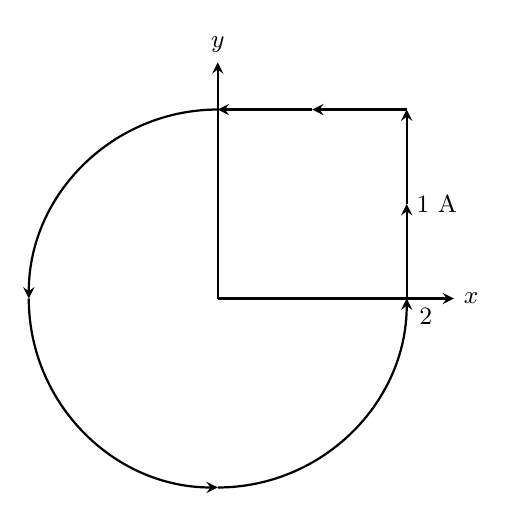
\begin{tikzpicture}[xscale=1.2,yscale=1.2,font=\small]
	\def\XD{0cm}
	\def\YD{0cm}

	\draw[thick, ->, >=stealth] (2cm, 0cm) -- (2cm, 1cm);
	\draw[thick, ->, >=stealth] (2cm, 1cm) -- (2cm, 2cm);
	\draw[thick, ->, >=stealth] (2cm, 2cm) -- (1cm, 2cm);
	\draw[thick, ->, >=stealth] (1cm, 2cm) -- (0cm, 2cm);
	\draw[thick, ->, >=stealth] (0,2cm)  arc (90:180:2); % -- (0cm, 0cm);
	\draw[thick, ->, >=stealth] (-2,0cm)  arc (180:270:2); % -- (0cm, 0cm);
	\draw[thick, ->, >=stealth] (0,-2cm)  arc (270:360:2); % -- (0cm, 0cm);
	%\node[above] at (0.75cm, 0.2cm){$60^0$};
	
	\coordinate[label=below:$2$] (x2) at (2.2cm,0cm);
	\coordinate[label=right:$1$ A] (1A) at (2cm,1cm);
	
	\draw[thick, ->, >=stealth] (0cm, 0cm) -- (0cm, 2.5cm);
	\coordinate[label=above:$y$] (y) at (0cm,2.5cm);
	\draw[thick, ->, >=stealth] (0cm, 0cm) -- (2.5cm, 0cm);
	\coordinate[label=right:$x$] (x) at (2.5cm,0cm);
\end{tikzpicture}
\end{figure}
\end{document}
